\section{Kategorisering}
Kategoriserings funktionen inddeles i klasser af typen boundary og en tilhørende controller, som det fremgår af \autoref{fig:DesignKategorisering}.

\begin{figure} [H]
\centering
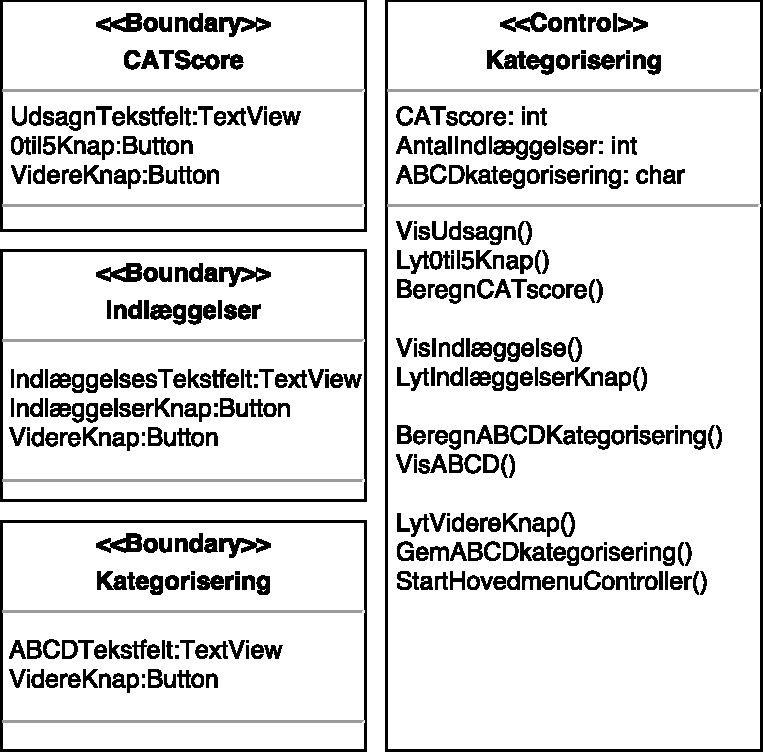
\includegraphics[width=0.9\textwidth]{figures/MVC/MVCKategorisering}
\caption{Designklasser for kategorisering.}
\label{fig:DesignKategorisering}
\end{figure}

\noindent
I \textit{KategoriseringGrænseflade} stilles otte udsagn fra CAT-scoren, som besvares af brugeren ved hjælp af knapper af typen button. Dertil fremgår der ligeledes en videre knap for således, at brugeren kan bekræfte sit svar og fortsætte til næste udsagn. Efter udsagnene er besvaret, skal indlæggelser det seneste år forårsaget af KOL besvares ud fra to yderligere knapper. Når kategoriseringen er beregnet vises denne i et tekstfelt. 

\textit{KategoriseringController} håndterer tryk af de forskellige knapper samt beregning af kategoriseringen ud fra den samlede CAT-score og antal indlæggelser. Kontrolleren lytter efter knapperne til besvarelse af de otte udsagn samt indlæggelser. Efter kategoriseringen er beregnet sendes denne til databasen, hvorefter den gemmes. Dertil har kontrolleren metoden til at starte hovedmenuen efter gennemført kategorisering.  